%*******************************************************************************
%*********************************** First Introduction *****************************
%*******************************************************************************
%\chapter{Introduction}  %Title of the First Introduction
%\chapter*{Introduction}
\chapter{Project Work}  %Title of the First Introduction
%\addcontentsline{tableofcontents}{chapter}{introduction}

\ifpdf
    \graphicspath{{Core/Figs/Raster/}{Core/Figs/PDF/}{Core/Figs/}}
\else
    \graphicspath{{Core/Figs/Vector/}{Core/Figs/}}
\fi

%********************************** %First Section  **************************************
\section{Data Collection} %Section - 1.1 
Our dataset is the Variome Corpus\cite{verspoor2013annotating}, which is openly accessible. \footnote{\href{http://www.opennicta.com.au/home/health/variome}\url{http://www.opennicta.com.au/home/health/variome}} \citet{verspoor2013annotating} gave a detailed illustration of the document selection and annotation process. I will summarize the main points here.\newline\newline
A major part of the current biomedical research lies in understanding the relations between human genetic variation and disease phenotypes. The \emph{Human Variome Project}, or \emph{HVP}, is a global initiative to collect all genetic variation information affecting human health\cite{ring2006human}. In particular, it acts as a liaison between individuals and organizations to integrate the genetic variants into databases that are open to the general public\cite{verspoor2013annotating}. The \emph{International Society for Gastrointestinal Hereditary Tumours (InSiGHT)}, is an international organization which aims to benefit patients with hereditary gastrointestinal(GI) tumours by research, education and personal assistance. In 2008, InSiGHT and HVP began a collaboration which propels InSiGHT to refine its process in the integration and interpretation of genetic variants. Consequently, a substantial effort was made to understand the mutation of mismatch repair(MMR) genes, the cause of Lynch Syndrome - one of the main syndromes of GI cancer\cite{silva2009mismatch}. A total of 10 full-text articles were selected from PubMed Central\textregistered  by searching the common Lynch syndrome genes. These documents cover inherited colon cancer as well as certain other cancers. The annotation schema, also known as the Variome Annotation Schema\cite{verspoor2013annotating}, include 11 entity types and 13 relation types, as can be seen in the table \ref{table:Variome_Relations}.\newline \newline
\begin{table}[h]
	\caption{Variome Relation Types}
	\centering
	\label{table:Variome_Relations}
	\begin{tabular}{|c | c |c  |}
		\hline 
		{Relation Type} 
		& Entity1 & Entity2\\ 
		\hline
		relatedTo  & mutation & disease \\
		relatedTo & disease & gene\\
		relatedTo & disease & body-part\\
		\hline 
		has     & gene & mutation\\
		has     & mutation & size\\
		has     & disease & characteristic\\
		has     & cohort-patient & age\\
		has     & cohort-patient & characteristic\\
		has     & cohort-patient & disease\\
		has     & cohort-patient & ethnicity\\
		has     & cohort-patient & gender\\
		has     & cohort-patient & mutation\\
		has     & cohort-patient & size \\
		\hline 
	\end{tabular}
\end{table}
In short, the annotation and selection of corpus is inspired by the needs of inSIGHT database, but intended for broader applications. In particular, the annotations are done by two human annotators. As suggested in \cite{verspoor2013annotating}, occasional annotation disagreement has been resolved and the result is merged into a single corpus. Thus in this relation extraction task here, we refer to the manual annotations as the gold standard. 
\section{Dependency Graph and Shortest Path}
	\begin{figure}[h]
		\centering
			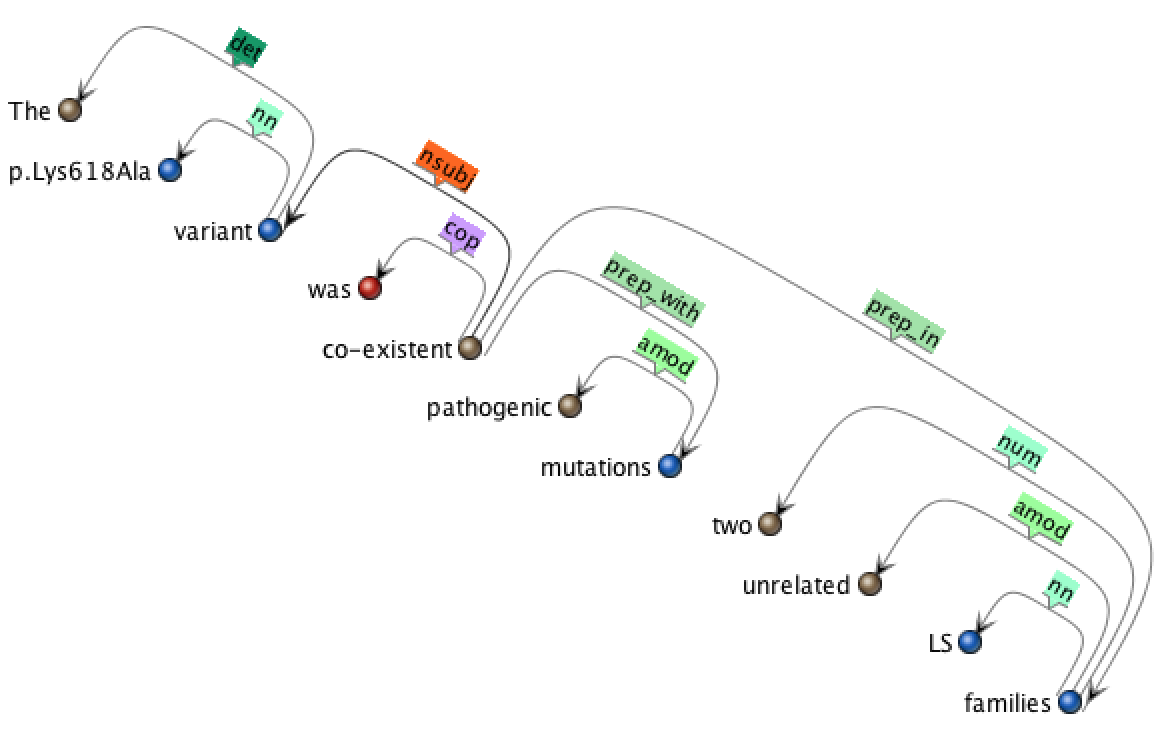
\includegraphics[width=\textwidth]{Dependency_Graph}
			\caption{Dependency Graph of `` The p.Lys618Ala variant was co-existent with pathogenic mutations in two unrelated LS families.''}
			\label{fig:Dependency_Graph}   
	\end{figure}
The dependency graph of a sentence is a directed graph, where nodes represent sentence tokens, and edges indicate their semantic relations. Figure \ref{fig:Dependency_Graph} shows the dependency graph of the sentence \emph{`` The p.Lys618Ala variant was co-existent with pathogenic mutations in two unrelated LS families.''} generated by the Stanford Parser. Such a graph preserves the rich semantic structure of a sentence, and has been widely regarded as an informative way of presenting a sentence. A detailed explanation of the relative constituents in the graph can be found in \cite{de2008stanford}. However, the point is to transfer only human-readable sentences to a computer-understandable data structure. The general idea would be to feed this graph into a learning algorithm and classify relations based on similarity to the sentence graph in the training set. Different approaches exist for this process. Turku Event Extraction System (TEES)\footnote{\href{https://github.com/jbjorne/TEES}https://github.com/jbjorne/TEES}, for instance, engineers a feature vector which consists of token features(part-of-speech tags and character constituents for each word), sentence features(bag-of-words counts), and graph-based features(dependency path represented as N-grams) and builds a multi-class SVM model with the feature vector\cite{bjorne2011generalizing}. In this project, we decide to use the \emph{Shortest Path Hypothesis}\cite{bunescu2005shortest}, namely the heuristic that the relation between two entities in a sentence can be distilled from the shortest path between these entities in the undirected version of the sentence dependency graph. This effectively reduces the burden of feature engineering\cite{liu2013approximate}, but it also calls for high-quality training data. We believe that with effective parameter tuning and clever graph matching techniques, the shortest path can be a single standalone feature for a relation between two entities.
\section{Approximate Subgraph Matching Algorithm}
\textbf{Disclaimer: As the Approximate Subgraph Matching system was originally developed for event extraction, it is more convenient to refer to the system as being learning ``events''. By nature events are nothing more than complex relations between entities, which is exactly the rationale behind adapting such an event extraction system for relations extraction tasks. What was later done in the adaptation process was treating relation as a type of ``event''. In this section, ``relations'' and ``events'' are used (somewhat) interchangeably. }\newline\newline
The Approximate Subgraph Matching framework, proposed by \citet{liu2013approximate} has the following work flow:
\subsection{Prepossessing}
As mentioned in section \ref{2.1}, in order to separate Named Entity Recognition from the Relation Extraction task, the named entity annotations are provided in training, development and test sets. The sentences are identified by the JULIE Sentence Boundary Detector\cite{tomanek2007sentence}, and parsed with the \emph{clearnlp} parser \footnote{\href{https://code.google.com/p/clearnlp/}https://code.google.com/p/clearnlp/}\cite{choi2013transition}. The model for dependency parsing and part-of-speech tagging is trained on the CRAFT corpus \cite{verspoor2012corpus}.
\subsection{Rule Learning}
	\begin{figure}[h]
		\centering
		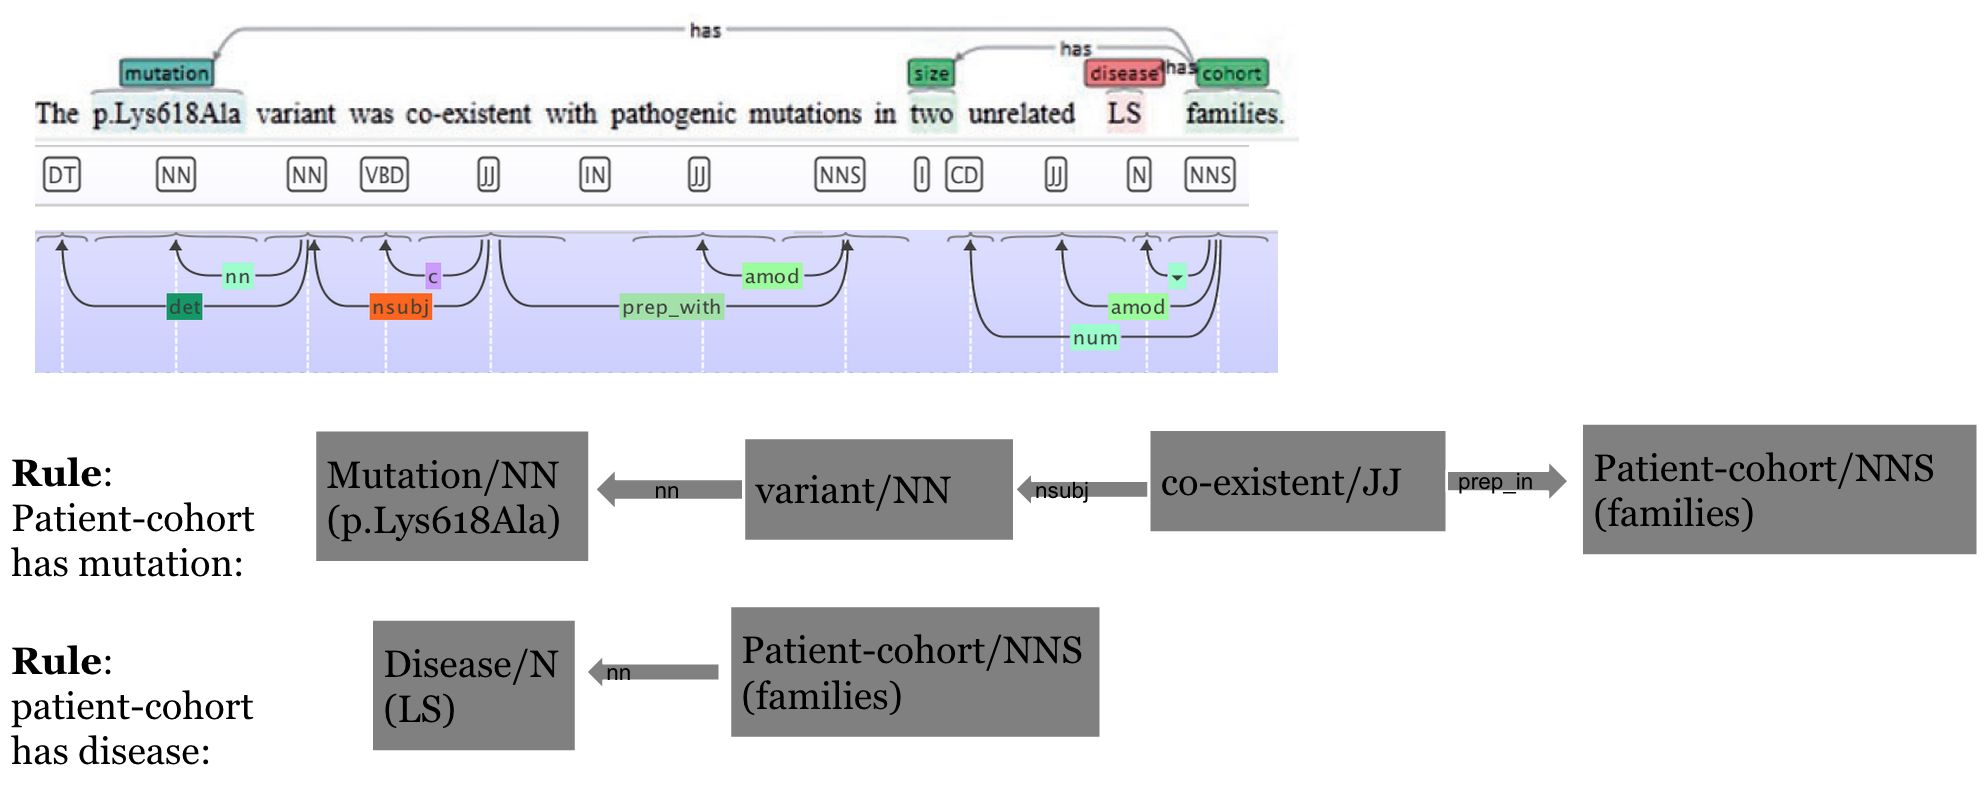
\includegraphics[width=\textwidth]{Rule}
		\caption{Rules learned for `` The p.Lys618Ala variant was co-existent with pathogenic mutations in two unrelated LS families.''}
		\label{fig:Rule}   
	\end{figure}
For each annotated sentence in the training set, a dependency graph is generated and the nodes representing entities are marked. The entity tokens are then replaced with their entity types, such that the rules learned are about an the generic entity types (e.g. gene mutation) instead of specific entities (e.g. p.Lys618Ala), so that our model has a better ability to generalize as we might not see the specific entities again in the test set. Next, the graph is transformed to its undirected version and the shortest path between entities are found with Dijkstra algorithm. This path is leaned as a rule associated with the event type in the annotation as a rule corresponding to that event type. Figure \ref{fig:Rule} gives an example of the learned rules for sentence \emph{`` The p.Lys618Ala variant was co-existent with pathogenic mutations in two unrelated LS families.''} This kind of instance-based learning can be effective provided there is enough training data\cite{alpaydin2014introduction}. A set of rules would then be learned for each event type, representing the graph patterns that indicating a specific type of event. 
\subsection{Sentence Matching}
The rules generated from the previous step could, in theory, be used to match sentences. For each sentence in the test set, a dependency graph can be generated together with the entity annotations(these are provided, as discussed). The graph can be searched exhaustively looking at the path(s) between each entity tokens, for an exact match with one or more rules within the rule set. This step is know as searching for exact subgraph isomorphism. Figure \ref{fig:ESM} gives an example of Exact Subgraph Matching(ESM).\newline\newline
\begin{figure}[h]
	\centering
	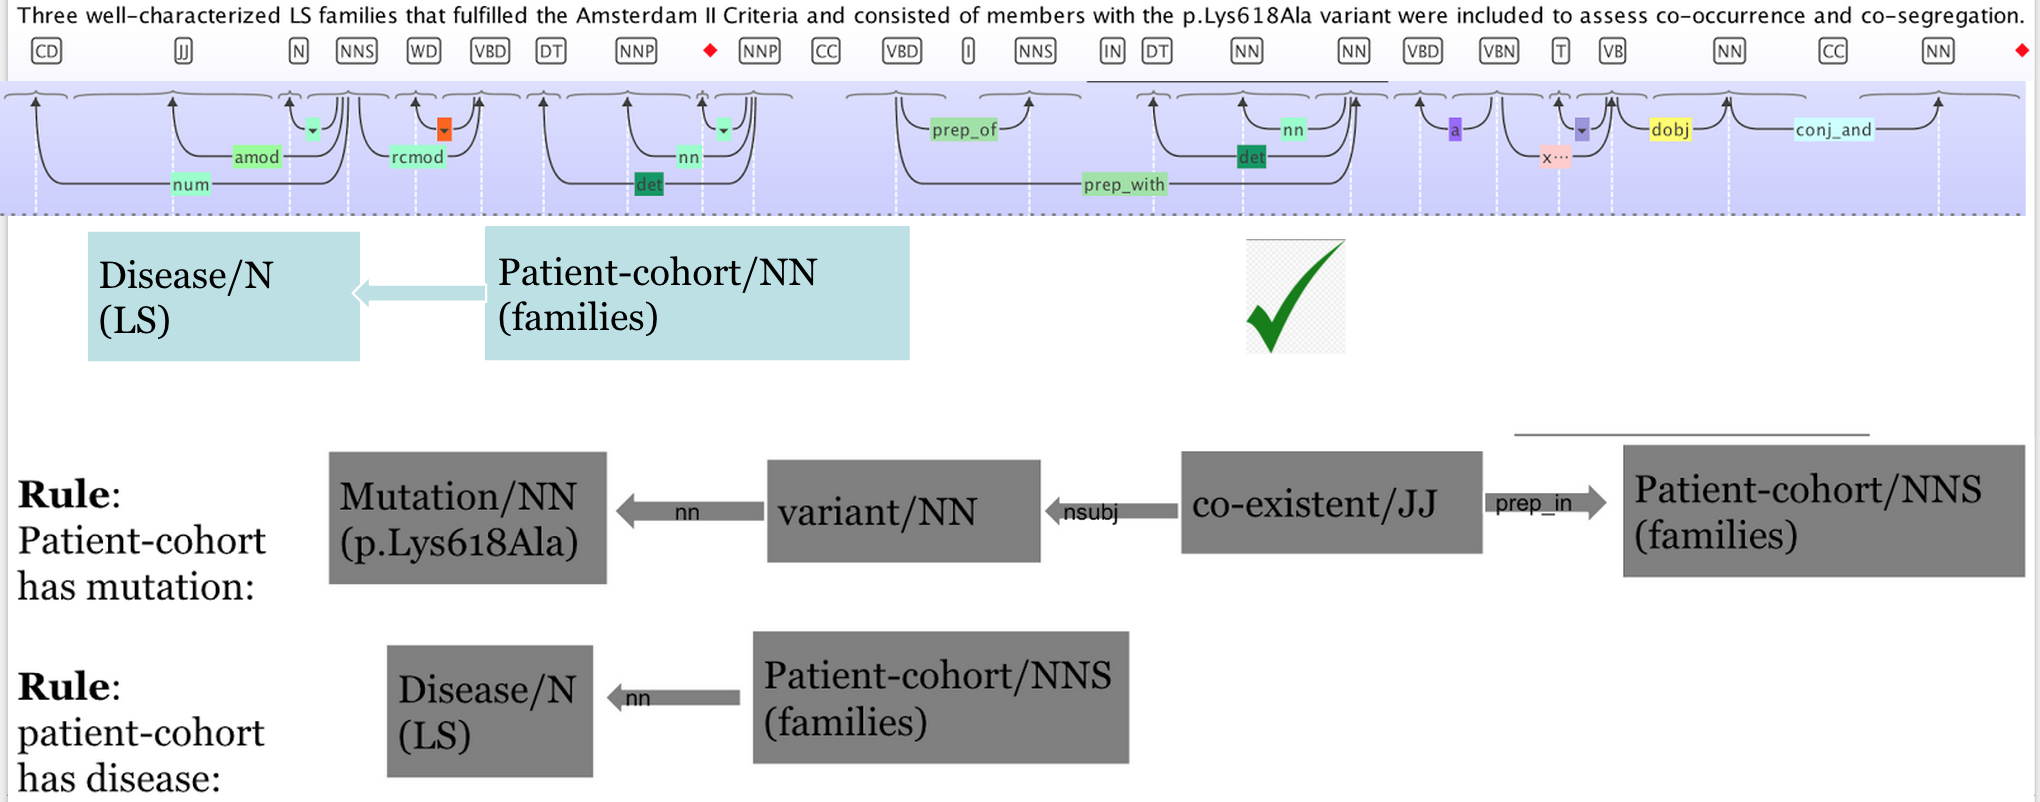
\includegraphics[width=\textwidth]{ESM}
	\caption{Exact Subgraph Matching}
	\label{fig:ESM}   
\end{figure}
However, the above-mentioned matching approach would invariably lead to low recall, as the richness of language can almost always produce slightly different dependency graph structure representing exactly the same events between the same entities. For instance, Figure \ref{fig:ASM} shows a scenario where \emph{patient-cohort has mutation} should be extracted as an event of interest, but there is a slight mismatch in the subgraph patterns. This leads to the rationale behind approximate subgraph matching, which relaxes the matching process and allows for a penalty-based matching. The formula for calculating subgraph distance is: 
\begin{equation}
\begin{split}
GraphDist(SentenceGraph, RuleGraph) = \\
w1 \times structDist(SentenceGraph, RuleGraph)  +\\ 
w2 \times labelDist(SentenceGraph, RuleGraph)   +\\
w3 \times directionalityDist(SentenceGraph, RuleGraph)\\
\end{split}
\end{equation}
$structDist$ is the structural difference between two subgraphs denoted by the distance between each pair of matched nodes. $labelDist$ and $directionalityDist$ are the difference in edge labels and edge directions respectively\cite{liu2013approximate}.
\begin{figure}[h]
	\centering
	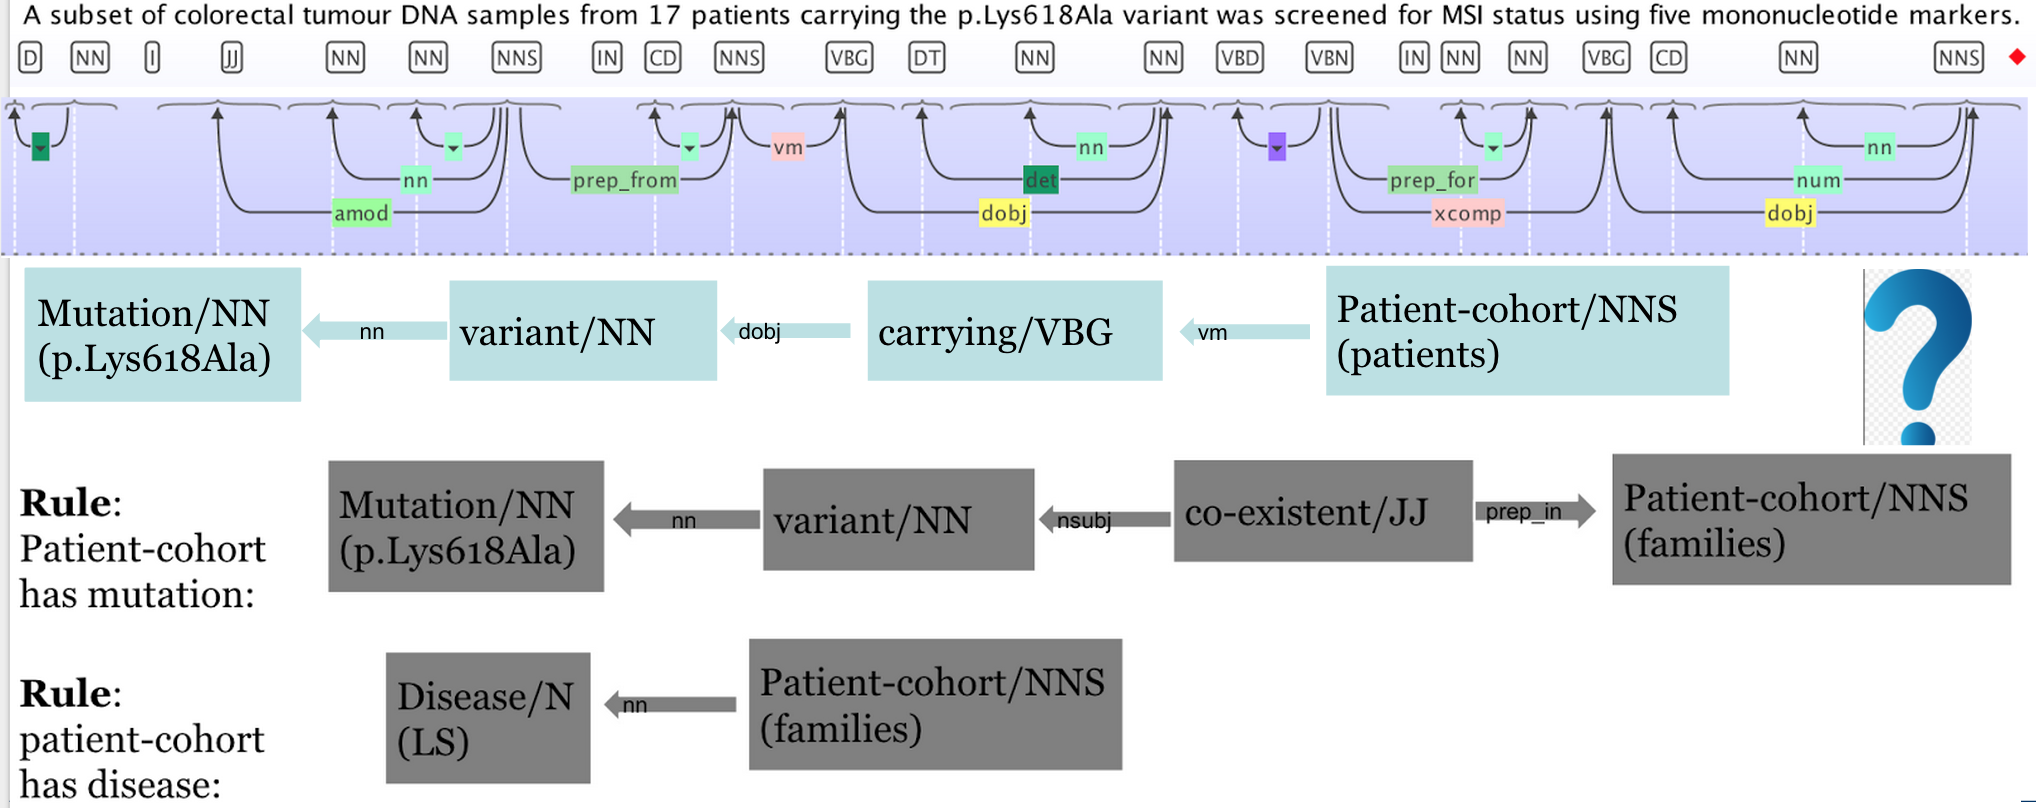
\includegraphics[width=\textwidth]{ASM}
	\caption{Approximate Subgraph Matching}
	\label{fig:ASM}   
\end{figure}
\subsection{Rule Optimization}
To avoid learning the idiosyncrasies in the training data, an iterative rule set optimization process is executed. After the initial learning phase, each rule in the rule set is tested first on the training data to see if it get produce accurate enough predictions (above 0.25). The low performing rules are discarded as a consequence.   
\section{System Adaptation}
\begin{figure}[h]
	\centering
	\begin{subfigure}[b]{0.3\textwidth}
		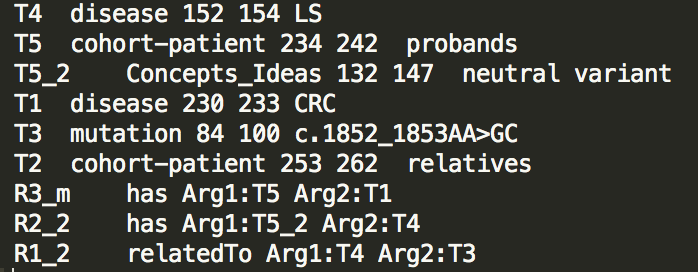
\includegraphics[width=\textwidth]{ann}
		\caption{before	: ann}
		\label{fig:ann}
	\end{subfigure}             
	\vfill
	\begin{subfigure}[b]{0.3\textwidth}
		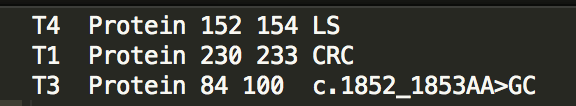
\includegraphics[width=\textwidth]{a1}
		\caption{after: a1}
		\label{fig:a1}   
	\end{subfigure}
	~
	\begin{subfigure}[b]{0.3\textwidth}
		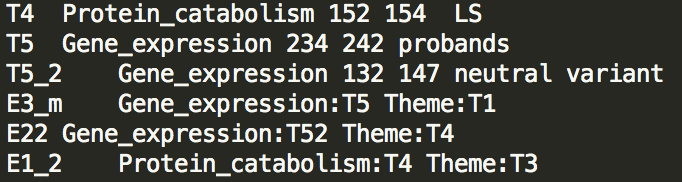
\includegraphics[width=\textwidth]{a2}
		\caption{after: a2}
		\label{fig:a2}   
	\end{subfigure}  
	\caption{Changing Annotation Format}
	\label{fig:annotation_format}
\end{figure}
As mentioned in \ref{section1.3}, the project aims at adapting an existing event extraction system on relation extraction tasks. The existing ASM system was developed for the BioNLP Shared Task 2011 and 2013.\newline\newline \emph{BioNLP shared Task} series is a community-wide text mining challenge specifically for biomedical literatures. The GE task in shared task 2013 aims at retrieving events of the following format: The \emph{.a1} files list all the entities as in Figure \ref{fig:a1}, the \emph{.a2} files list all the event triggers, followed by events as in Figure \ref{fig:a2}. An entity is annotated with its ID, entity type, text offsets, and the textual token. The same goes for triggers. Events are annotated as a relation between the event trigger and one or more entities.\newline\newline
Figure \ref{fig:ann} shows the \emph{Variome Annotation Format}. Different from the shared task, all the annotations would be in one \emph{.ann} file, with entities annotated the same way as in the shared task, and relations similar to events. However, relations do not have triggers at all. This distinction became a major challenge for this project. During the duration of this project, most of my attempts to fully adapt the system to relation extraction tasks have failed. In essence, the differentiation in the retrieval process lies in the event retrieval relies on the detection and prediction of a trigger word, where as the relation extraction does not. \newline\newline
My only attempts that worked was transforming the annotation format of the Variome Corpus to that of the BioNLP Shared Task 2013, such that the original system would not break. The transformation is illustrated in this tables. The "has" relationship is transformed to "gene regulation" event, and "relatedTo" relationship is transformed to "Phosphyrilation" event, with the entity annotation slightly too. The entities would be of type "Protein" instead of the original entity types in the Variome Corpus. \textbf{The major bottleneck for this adaptation work is that the original system includes a hard-coded trigger detection and prediction process.} As for events detecting trigger words such as "activates" for gene expression is an important step for prediction. However, this process is not included at all in the event prediction process and to cope with the original system I had to add "fake triggers" for these events. As a result, the first entity of each event/relation annotation is added as the trigger for the notation. \newline\newline
As shown in Figure \ref{fig:annotation_format}, the original Variome Annotation file (.ann) is splitted into two files(.a1 and .a2), The code checks if the entity exist in any event annotations. If not, the annotation will be ignored such as $T2$. Next the code checks if the annotation is a first argument or second argument. If the annotation is the first argument, it is treated as an event trigger, such as $T4, T5, T5\_2$. The trigger annotations are above the event annotations in the .a2 file where as the other entity annotations are in the .a2 file. 
After this first attempt I had a few better ideas to add fake triggers, the best one being adding the entity types (patient-cohort), with parenthesis directly after the entity tokens and do a binding event. Due to the time constraints and these ideas being essentially fool's gold, I did not implement these ideas.

\section{Results}
\begin{table}[h]
	\caption{Overall Result}
	\centering
	\label{table:overall_result}
	\begin{tabular}{|c | c c |c c c c |}
		\hline 
		{Relation Type} 
		& Gold & Answer  & Match  & Precision & Recall & F1-score\\ 
		\hline
		has  & 1711 & 1310 & 402 & 0.3069 & 0.2350 & 0.2661 \\
		
		relatedTo & 157 & 1498 &  36 & 0.0240 & 0.2293 & 0.0435\\
		\hline 
		TOTAL  & 1868 & 2808 & 438 & 0.1560 & 0.2345 & 0.1874 \\
		\hline 
	\end{tabular}
\end{table}
The overall result of the system is shown in table \ref{table:overall_result}, the main reason the system is not performing well is that it is not predicting the triggers words correctly, because I have chosen to treat entity annotations as triggers. Trigger prediction is usually treated as a classification problem where for every token in the test sentence, a score is assigned for labeling it as trigger for each event type. 

Another important reason is the entity type is quite different from the proteins as proclaimed. 